\documentclass[12pt]{beamer}

\usetheme{Oxygen}
\usepackage{thumbpdf}
\usepackage{wasysym}
\usepackage{ucs}
\usepackage[utf8]{inputenc}
\usepackage{pgf,pgfarrows,pgfnodes,pgfautomata,pgfheaps,pgfshade}
\usepackage{verbatim}
\usepackage[spanish]{babel}
\usepackage{listings}

\lstdefinelanguage{uuagc}                   % name language
                  []{haskell}               % base language
                  {morekeywords={ATTR       % language keywords            
                                ,SEM
                                ,DATA
                                ,TYPE
                                ,lhs
                                ,loc
                                }
                  ,sensitive=true           % syntax sentitive
                  ,morestring=[d]"          % string delimiters
                  ,morestring=[d]'
                  }

\lstnewenvironment{ag}{\lstset{ language=uuagc
                              , identifierstyle=\ttfamily
                              , showstringspaces=false
                              , basicstyle=\scriptsize
							  , keepspaces=true
                              , stringstyle=\scriptsize
                              , extendedchars=true
                              , commentstyle=\color{blue}
                      }
                      }{}
\lstnewenvironment{hs}{\lstset{ language=haskell
                              , identifierstyle=\ttfamily
                              , showstringspaces=false
							  , basicstyle=\scriptsize
							  , keepspaces=true
                              , stringstyle=\scriptsize
                              , extendedchars=true
                              , commentstyle=\color{blue}
                      }
                  }{}

\setbeamertemplate{navigation symbols}{\insertslidenavigationsymbol}



\pdfinfo
{
  /Title       (Desarrollo de Navegador Web con Haskell)
  /Creator     (TeX)
  /Author      (Carlos Gomez)
}


\title[Defensa de Proyecto de Grado]{
\textbf{\large DESARROLLO DE NAVEGADOR WEB}\\
\textbf{\large CON}\\
\textbf{\large HASKELL\footnote{\tiny Defensa de Proyecto de Grado, 
Presentado para Optar al Diploma Académico de Licenciatura en Informática}}
}

%\subtitle{subtitulo}
\author{Carlos Gomez}

\institute[UMSS]{
	Universidad Mayor de San Simón\\
	Facultad de Ciencias y Tecnología\\
	Carrera de Licenciatura en Informática}

\date{11 de Julio, 2011}

\begin{document}

\frame{\titlepage}

\section*{}
\begin{frame}
  \frametitle{Contenido}
  \tableofcontents[section=1,hidesubsections]
\end{frame}

%\AtBeginSection[]
%{
%  \frame<handout:0>
%  {
%    \frametitle{Contenido}
%    \tableofcontents[currentsection,hideallsubsections]
%  }
%}

%\AtBeginSubsection[]
%{
%  \frame<handout:0>
%  {
%    \frametitle{Contenido}
%    \tableofcontents[sectionstyle=show/hide,subsectionstyle=show/shaded/hide]
%  }
%}

\newcommand<>{\highlighton}[1]{%
  \alt#2{\structure{#1}}{{#1}}
}

\newcommand{\icon}[1]{\pgfimage[height=1em]{#1}}



%%%%%%%%%%%%%%%%%%%%%%%%%%%%%%%%%%%%%%%%%
%%%%%%%%%% Content starts here %%%%%%%%%%
%%%%%%%%%%%%%%%%%%%%%%%%%%%%%%%%%%%%%%%%%

\section{Introducción}

\begin{frame}
\begin{center}
	\textbf{\Large Introducción}
\end{center}
\end{frame}

\subsection{Navegadores Web}

\begin{frame}
\frametitle{Navegadores Web}
	\begin{itemize}
		\item Programa informático del lado del cliente, que se encarga de renderizar documentos.
		\item Trabaja con varias tecnologías y estándares Web:
		\begin{itemize}
			\item HTML/XHTML/XML
			\item CSS
			\item DOM
			\item JavaScript
			\item ..., etc.
		\end{itemize}
	\end{itemize}
\end{frame}

\begin{frame}
\frametitle{Navegadores Web Actuales}
	\begin{figure}
		\scalebox{0.15}{
\includegraphics{graphics/navegadores.jpg}}
	\end{figure}

	Fueron desarrollados con lenguajes de programación imperativos.

	\begin{tabular}[]{|l|l|p{5cm}|} \hline
	\textbf{Motor de Rend.} &	\textbf{Leng. Prog.}	&	\textbf{Navegadores Web} \\
	\hline
	Gecko					&	C$++$					&	Firefox, Camino, Flock, 
															SeaMonkey,	K-Melen, Netscape 9, 
															Lenascape, Epiphany \\
	%\hline
	%Trident					&	COM\footnote{\tiny Component Object Model}/IDL
	%													&	Internet Explorer	\\
	\hline
	Presto					&	C$++$					&	Opera	\\
	\hline
	WebKit					&	C$++$					&	Safari, Google Chrome \\
	\hline
	\end{tabular}
	{\tiny Fuente: Wikipedia}
\end{frame}

\begin{frame}[fragile]
\frametitle{Lenguajes Imperativos vs Funcionales}

Los programas gigantes (Navegadores Web) \highlighton{exigen} que el lenguaje de programación
permita un \highlighton{alto nivel de modularidad, código compacto, fácil de comprender}, etc,
con el objetivo de reducir el costo de desarrollo del programa.

\begin{tabular}[c]{|p{3cm}|c|c|} \hline
							&	\textbf{Prog. Imperativa}		&		\textbf{Prog. Funcional}	\\
\hline
\textbf{Navegadores Web
	    Actuales}			&   \scalebox{0.05}{
\includegraphics{graphics/Ok.png}}
																&	WWWBrowser 
																	\scalebox{0.15}{
\includegraphics{graphics/pregunta.jpg}}
																									\\ 
\hline
\end{tabular}

\begin{block}{}
Los lenguajes funcionales, en muchos casos, permiten aprovechar \highlighton{estas caracteristicas} al maximo
y reducir el costo de desarrollo. Pero no existe un Navegador Web actual implementado en un lenguaje de programación
funcional.
\end{block}
\end{frame}




\begin{frame}
\frametitle{Haskell}
\begin{center}
	\scalebox{0.4}{
\includegraphics{graphics/HaskellLogo.png}}
\end{center}

\begin{block}{Haskell}
\textbf{Haskell} es un lenguaje de programación funcional, con evaluación perezosa y de 
propósito general \highlighton{que incorpora muchas de las innovaciones recientes del diseño de lenguajes
de programación.}
\begin{flushright}
\--- \textit{(Peyton Jones, Haskell 98 Report, 2002)}
\end{flushright}
\end{block}
\end{frame}

\subsection{Motivación del Proyecto}
\begin{frame}
\frametitle{Motivación del Proyecto}

\begin{block}{Motivación del Proyecto}
Experimentar las capacidades/características, librerías y herramientas
de Haskell en el Desarrollo de un Navegador Web.
\end{block}

\end{frame}

\subsection{Objetivos del Proyecto}
\begin{frame}
\frametitle{Objetivos del Proyecto}

\begin{block}{Objetivo General}
Desarrollar un Navegador Web con el lenguaje de programación funcional Haskell.\\
\end{block}

\begin{block}{Objetivos Específicos}
\begin{itemize}
	\item Desarrollar el módulo de comunicación entre el Navegador Web y los
	protocolos HTTP y modelo TCP/IP.
	\item Desarrollar un intérprete de la información HTML.
	\item Desarrollar algoritmos que permitan mostrar la información en la pantalla
	del Navegador Web.
	\item Desarrollar la Interfaz Gráfica de Usuario (GUI).
	\item Desarrollar un módulo que dé soporte a CSS (Cascading Style Sheet).
\end{itemize}
\end{block}

\end{frame}


\section[Desarrollo]{Desarrollo del Proyecto}

\begin{frame}
\begin{center}
	\textbf{\Large Desarrollo del Proyecto}
\end{center}
\end{frame}

\subsection{Principales Herramientas y Librerías}
\begin{frame}
\frametitle{Principales Herramientas y Librerías}
Principales Herramientas y Librerías que se utilizaron en el proyecto:

\begin{itemize}
	\item Librería uu-parsinglib
%	Librería EDSL\footnote{Embded Domain Specific Language} para Haskell que
%	permite procesar una entrada a través de una descripción similar a la sintaxis 
%	concreta de un lenguaje.
	\item Herramienta UUAGC
%	Herramienta que genera código Haskell a través de una descripción de gramática
%	de atributos de un comportamiento.
	\item Librería wxHaskell
%	Librería gráfica para Haskell que permite implementar el GUI de un programa.
	\item Librería libcurl
%	Librería para interactuar con los protocolos HTTP, File, FTP, etc.
	\item Librería Map
%	Librería para manipular una lista de elementos clave-valor.
\end{itemize}
\end{frame}

\subsection{Renderización de un documento}

\begin{frame}
\frametitle{Renderización}
La renderización consiste en convertir un documento de texto (descrito por un
lenguaje de marcado) a un formato visual en la pantalla.

\begin{figure}
	\scalebox{0.35}{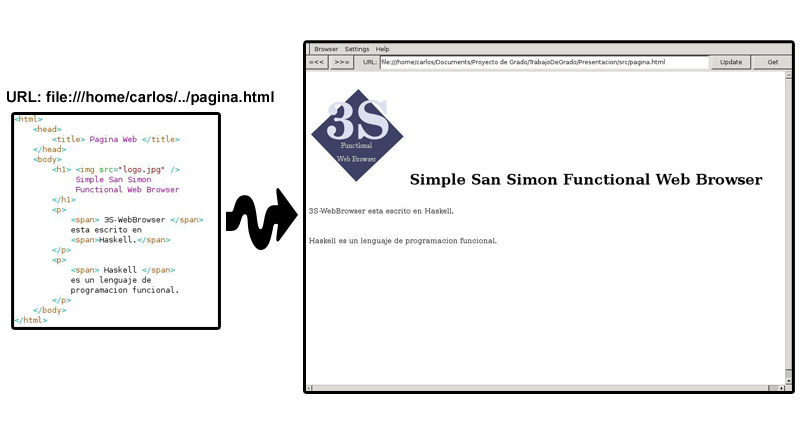
\includegraphics{graphics/renderizacion.jpg}}
\end{figure}
\end{frame}

\begin{frame}
\frametitle{Renderización}
La renderización es realizada aplicando un conjunto de transformaciones a la entrada
hasta obtener un formato visual para la pantalla.

\begin{figure}
	\scalebox{0.35}{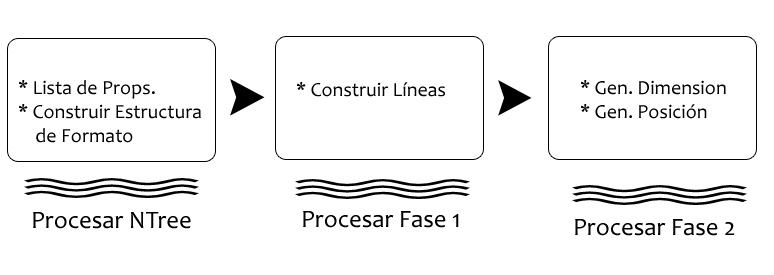
\includegraphics{graphics/transformTree.jpg}}
\end{figure}
\end{frame}

\subsubsection{Diagrama de Renderización}
\begin{frame}
\frametitle{Diagrama de Renderización}
\framesubtitle{Estado inicial + GUI con wxHaskell}
	\scalebox{0.35}{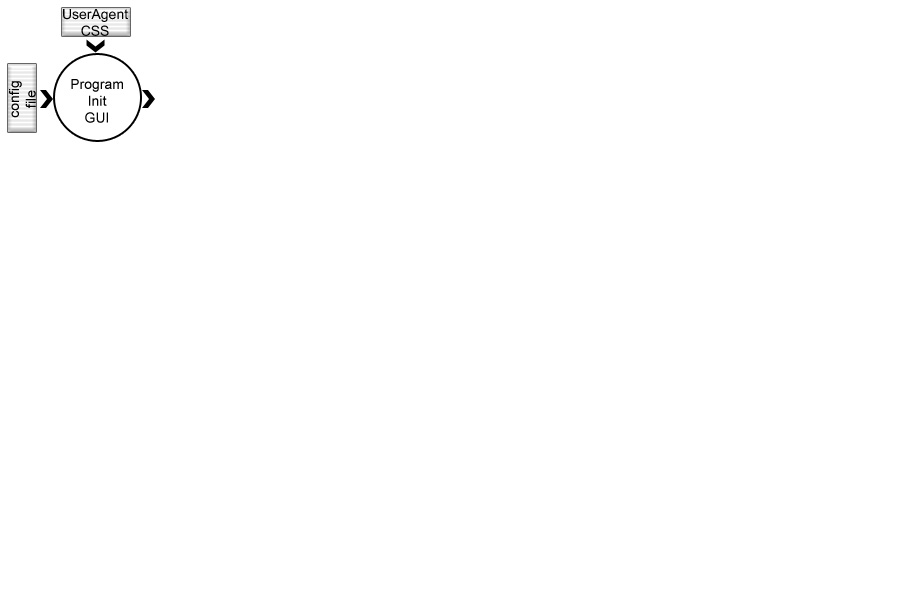
\includegraphics{graphics/rend/1.jpg}}
\end{frame}

\begin{frame}
\frametitle{Diagrama de Renderización}
\framesubtitle{Obtener el doc. y recursos con libcurl}
	\scalebox{0.35}{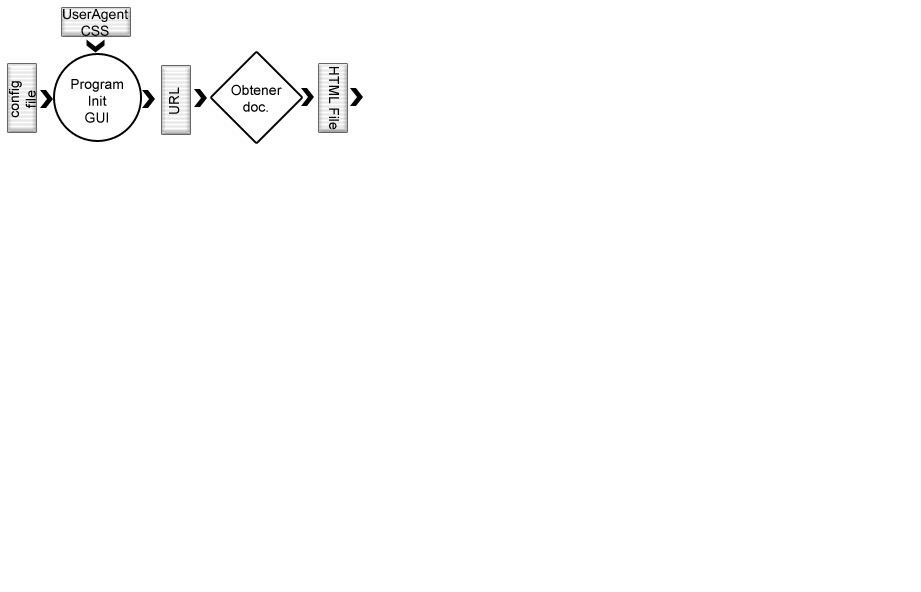
\includegraphics{graphics/rend/2.jpg}}
\end{frame}

\begin{frame}
\frametitle{Diagrama de Renderización}
\framesubtitle{Reconocer la entrada con uu-parsinglib}
	\scalebox{0.35}{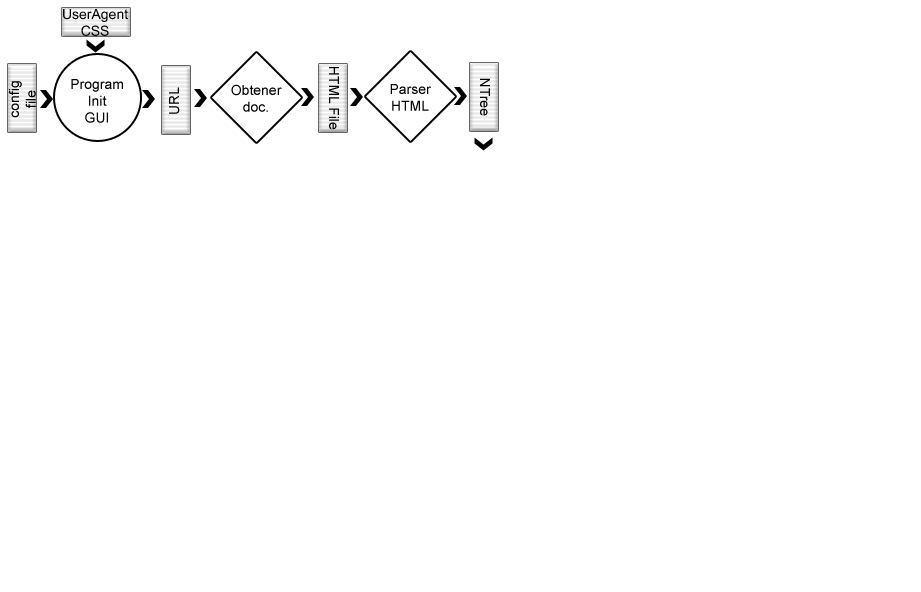
\includegraphics{graphics/rend/3.jpg}}
\end{frame}

\begin{frame}
\frametitle{Diagrama de Renderización}
\framesubtitle{Procesar el NTree con UUAGC}
		\scalebox{0.35}{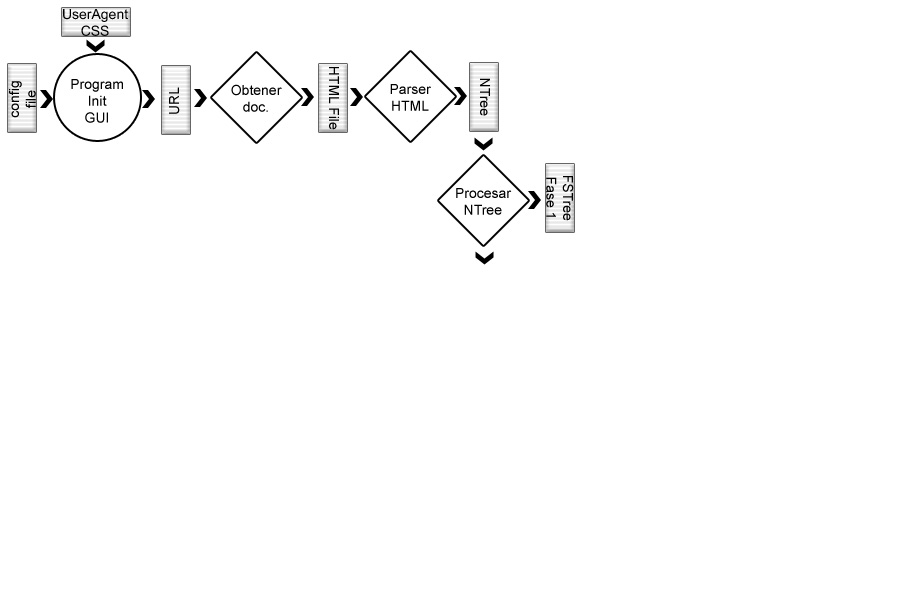
\includegraphics{graphics/rend/4.jpg}}
\end{frame}

\begin{frame}
\frametitle{Diagrama de Renderización}
\framesubtitle{Procesar el FSTreeFase1 con UUAGC}
	\scalebox{0.35}{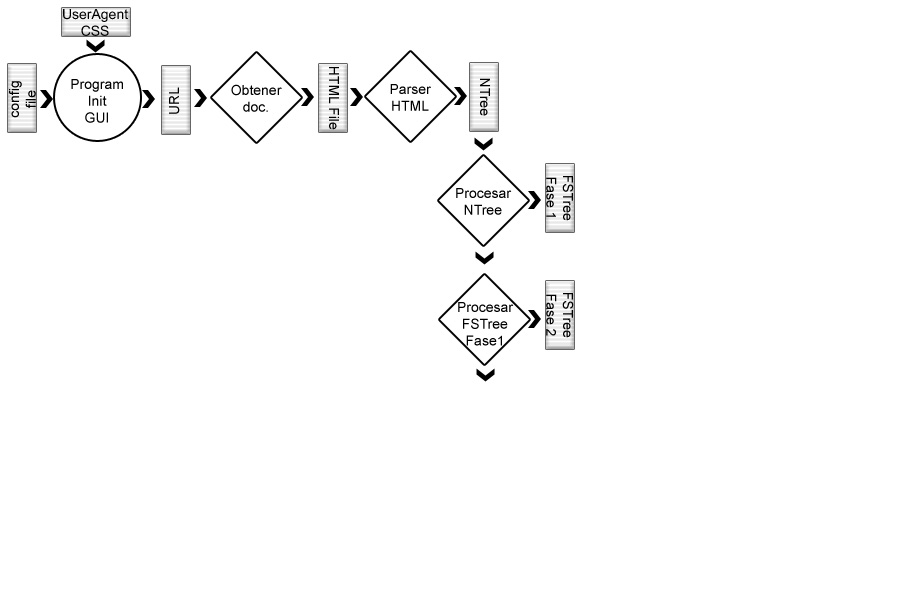
\includegraphics{graphics/rend/5.jpg}}
\end{frame}

\begin{frame}
\frametitle{Diagrama de Renderización}
\framesubtitle{Procesar el FSTreeFase2 con UUAGC}
	\scalebox{0.35}{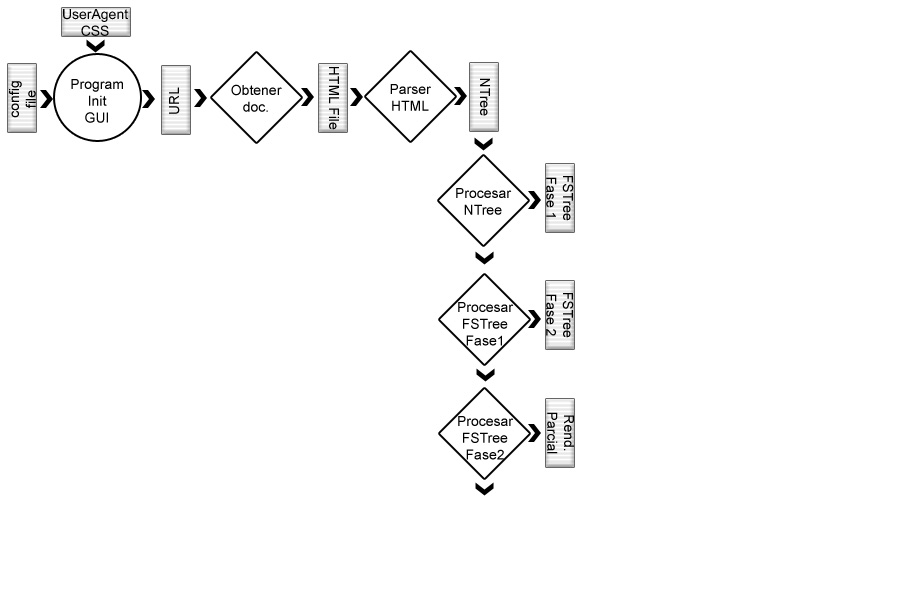
\includegraphics{graphics/rend/6.jpg}}
\end{frame}

\begin{frame}
\frametitle{Diagrama de Renderización}
\framesubtitle{Renderizar el documento y Props con wxHaskell}
	\scalebox{0.35}{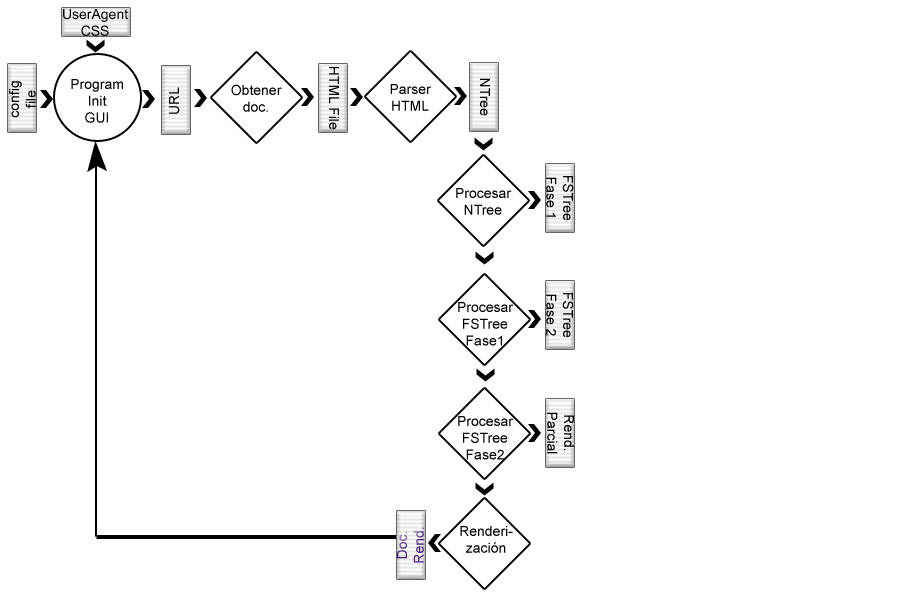
\includegraphics{graphics/rend/7.jpg}}
\end{frame}

\begin{frame}
\frametitle{Diagrama de Renderización}
\framesubtitle{Transformaciones}
	\scalebox{0.35}{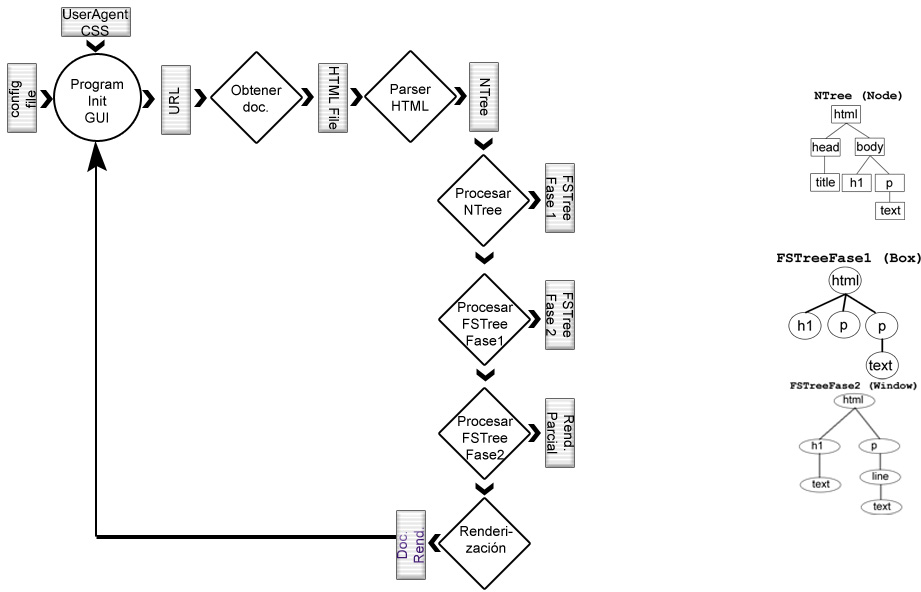
\includegraphics{graphics/rend/8.jpg}}
\end{frame}

\begin{frame}
\frametitle{Diagrama de Renderización}
\framesubtitle{Procesar NTree en detalle}
	\scalebox{0.35}{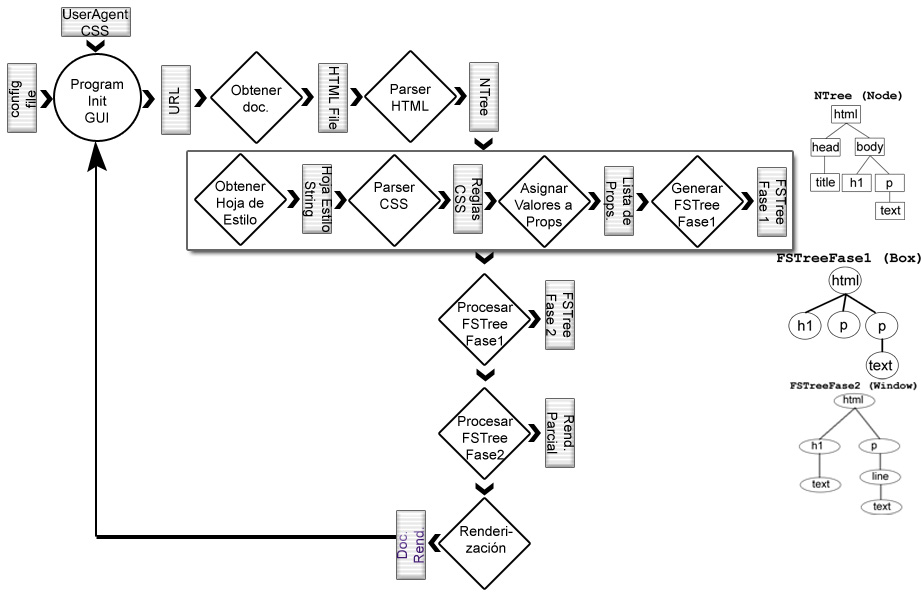
\includegraphics{graphics/rend/9.jpg}}
\end{frame}

\begin{frame}
\frametitle{Diagrama de Renderización}
\framesubtitle{Procesar FSTreeFase1 en detalle}
	\scalebox{0.35}{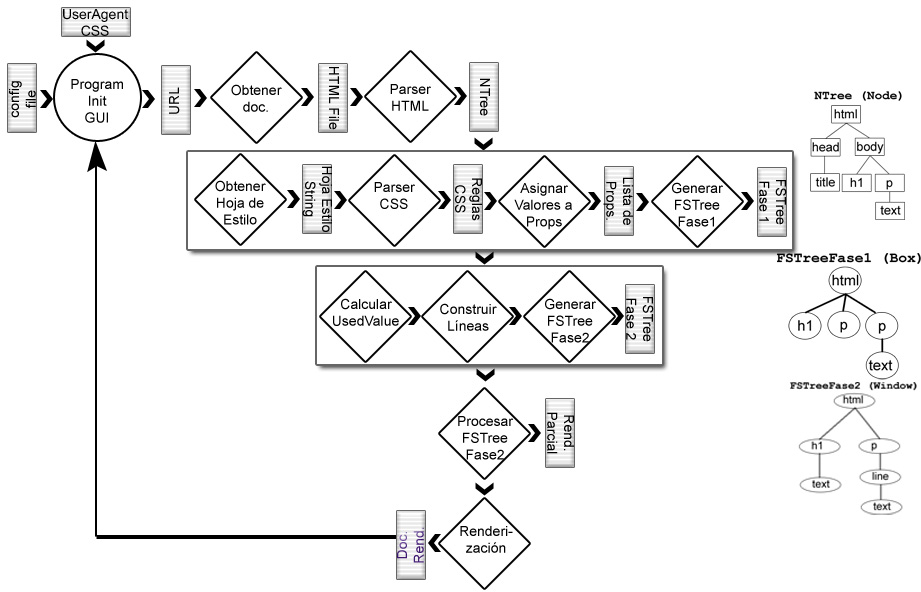
\includegraphics{graphics/rend/10.jpg}}
\end{frame}

\begin{frame}
\frametitle{Diagrama de Renderización}
\framesubtitle{Procesar FSTreeFase2 en detalle}
	\scalebox{0.35}{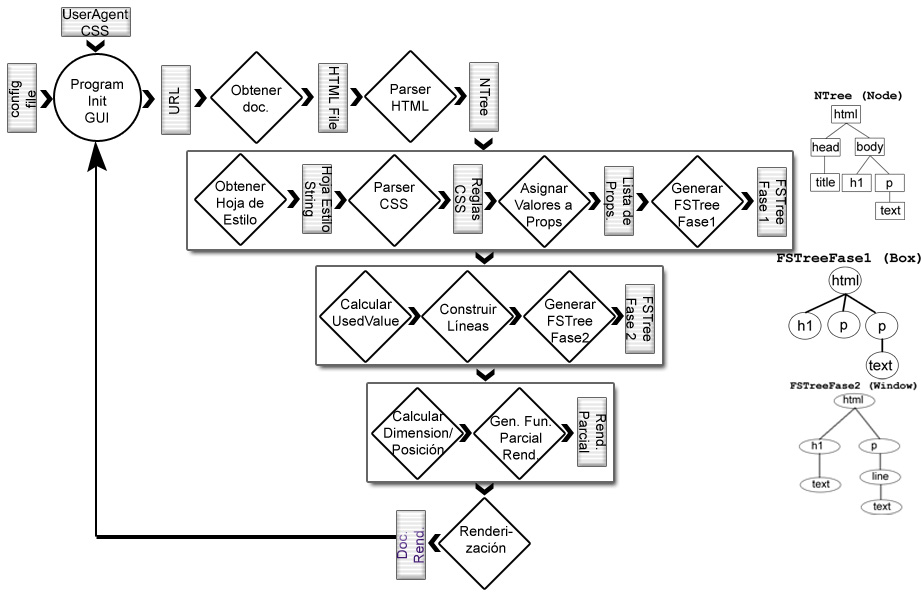
\includegraphics{graphics/rend/11.jpg}}
\end{frame}

\begin{frame}
\frametitle{Diagrama de Renderización}
\framesubtitle{Redimensionamiento de paginas}
	\scalebox{0.35}{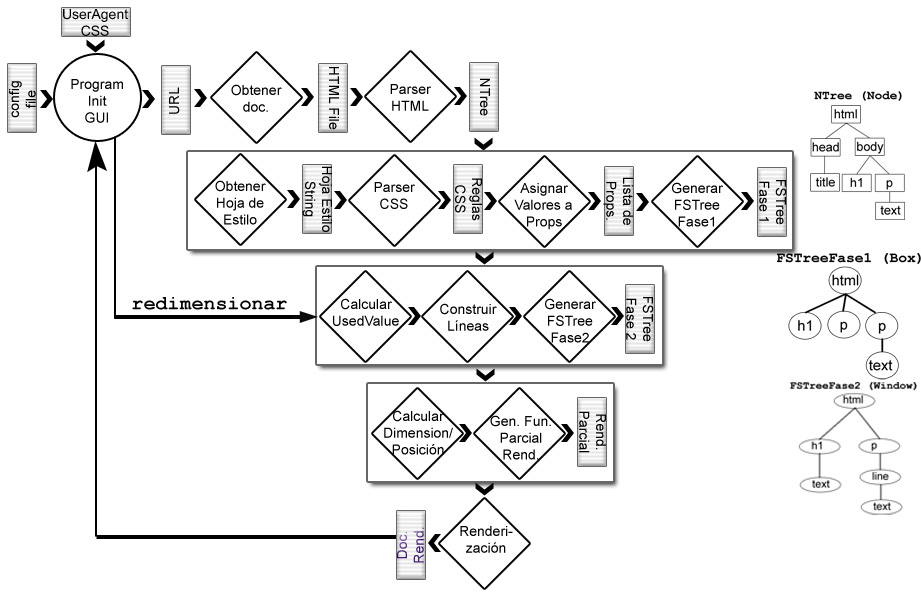
\includegraphics{graphics/rend/12.jpg}}
\end{frame}

\subsection{Tipos de Datos}

\subsubsection{NTree}
\begin{frame}[fragile]
\frametitle{NTree}
\framesubtitle{Estructura Rosadelfa (NTree)}
\begin{block}{}
\begin{ag}
DATA NTree
  | NTree Node ntrees: NTrees

TYPE NTrees = [NTree]

DATA Node
  | NTag   name     : String
           replaced : Bool
           atribs   : {Map.Map String String}
  | NText  text     : String
\end{ag}
\end{block}
\end{frame}

\subsubsection{FSTreeFase1}
\begin{frame}[fragile]
\frametitle{FSTreeFase1}
\framesubtitle{Estructura de formato de fase 1}
\begin{block}{}
\begin{ag}
DATA BoxTree
  | BoxContainer name : String
                 fcnxt: {FormattingContext}
                 props: {Map.Map String Property}
                 attrs: {Map.Map String String}
                 bRepl: Bool
                 boxes: Boxes
  | BoxText name : String
            props: {Map.Map String Property}
            attrs: {Map.Map String String}
            text : String
  | BoxItemContainer props: {Map.Map String Property}
                     attrs: {Map.Map String String}
                     boxes: Boxes

TYPE Boxes = [BoxTree]

DATA FormattingContext
  | InlineContext | BlockContext | NoContext
\end{ag}
\end{block}
\end{frame}

\subsubsection{FSTreeFase2}
\begin{frame}[fragile]
\frametitle{FSTreeFase2}
\framesubtitle{Estructura de formato de fase 2}
\begin{block}{}
\begin{ag}
DATA WindowTree
  | WindowContainer name : String
                    fcnxt: {FormattingContext}
                    props: {Map.Map String Property}
                    attrs: {Map.Map String String}
                    tCont: {TypeContinuation}
                    bRepl: Bool
                    elem : Element
  | WindowText name : String
               props: {Map.Map String Property}
               attrs: {Map.Map String String}
               tCont: {TypeContinuation}
               text : String
  | WindowItemContainer marker    : {ListMarker}
                        sizeMarker: {(Int,Int)}
                        elem      : Element
                        props     : {Map.Map String Property}
                        attrs     : {Map.Map String String}

DATA TypeContinuation 
  | Full  | Init  | Medium | End

\end{ag}
\end{block}
\end{frame}

\begin{frame}[fragile]
\frametitle{FSTreeFase2}
\framesubtitle{Estructura de formato de fase 2 (Continuación)}
\begin{block}{}
\begin{ag}
DATA Element
  | EWinds winds: WindowTrees
  | ELines lines: Lines
  | ENothing

TYPE WindowTrees = [WindowTree]

TYPE Lines       = [Line]

DATA Line
  | Line winds: WindowTrees

DATA ListMarker
  | Glyph      name : String
  | Numering   value: String
  | Alphabetic value: String
  | NoMarker
\end{ag}
\end{block}
\end{frame}

\subsection{CSS}
\begin{frame}
\frametitle{CSS}
\framesubtitle{Cascading Style Sheet (CSS)}
La especificación de CSS provee:
\begin{enumerate}
	\item Modelos para renderización
	\item Lenguaje para Hojas de Estilos
	\item Propiedades de CSS
\end{enumerate}
\end{frame}

\begin{frame}[fragile]
\frametitle{Modelo en Cascada}
\begin{itemize}
\item 3 Usuarios/Origen de donde provienen las hojas de estilo:
\begin{block}{}
\begin{ag}
DATA Origen
  | UserAgent | User | Author

\end{ag}
\end{block}

\item 3 Tipos de Hojas de estilo
\begin{itemize}
	\item \textbf{Externa}, elemento \textit{link} de HTML.
	\item \textbf{Interna}, elemento \textit{style} de HTML.
	\item \textbf{Atributos}, atributo \textit{style} de HTML.
\end{itemize}
\begin{block}{}
\begin{ag}
DATA Tipo
  | HojaExterna | HojaInterna | EstiloAtributo

\end{ag}
\end{block}
\item El usuario \textit{Author} es el único que puede definir estilos
en los 3 tipos. Los demás sólo pueden definir estilos del tipo externo.
\end{itemize}
\end{frame}

\begin{frame}[fragile]
\frametitle{Lenguaje para Hojas de Estilos}
Su representación es:
\begin{block}{}
\begin{ag}
TYPE HojaEstilo = [Regla]

TYPE Regla = (Tipo, Origen, Selector, Declaraciones)

DATA Selector
  | SimpSelector SSelector
  | CompSelector SSelector 
                 operador: String
                 Selector

DATA SSelector
  | TypeSelector nombre: String
                 Atributos 
                 MaybePseudo
  | UnivSelector Atributos MaybePseudo
\end{ag}
\end{block}
\end{frame}

\begin{frame}[fragile]
\frametitle{Lenguaje para Hojas de Estilos}
\begin{block}{}
\begin{ag}
TYPE Atributos = [Atributo]

DATA Atributo
  | AtribID     id: String
  | AtribNombre nombre: String
  | AtribTipoOp nombre, op, valor : String

TYPE MaybePseudo = MAYBE PseudoElemento

DATA PseudoElemento
  | PseudoBefore
  | PseudoAfter

TYPE Declaraciones = [Declaracion]

DATA Declaracion 
  | Declaracion nombre: String Value importancia: Bool
\end{ag}
\end{block}
\end{frame}

\begin{frame}[fragile]
\frametitle{Propiedades de CSS}
Existe como 80 propiedades para la pantalla, que se encuentran en la especificación de CSS.
Haskell permite representarlos casi de forma plana y directa.

\begin{block}{}
\begin{hs}
data Property 
  = Property { name           :: String
             , inherited      :: Bool
             , initial        :: Value
             , value          :: Parser Value
             , propertyValue  :: PropertyValue
             , fnComputedValue:: FunctionComputed
             , fnUsedValue    :: FunctionUsed }

data PropertyValue
  = PropertyValue { specifiedValue :: Value
                  , computedValue  :: Value
                  , usedValue      :: Value
                  , actualValue    :: Value }
\end{hs}
\end{block}
\end{frame}

\begin{frame}[fragile]
\frametitle{Propiedades de CSS (Continuación)}
El tipo de dato Value:
\begin{block}{}
\begin{ag}
DATA Value
  | PixelNumber   Float
  | PointNumber   Float
  | EmNumber      Float
  | Percentage    Float
  | KeyValue      String
  | KeyColor      rgb: {(Int,Int,Int)}
  | StringValue   String
  | ListValue     values: {[Value]}
  ...
  | NotSpecified
\end{ag}
\end{block}
\end{frame}

\begin{frame}[fragile]
\frametitle{Propiedades de CSS (Continuación)}
\begin{block}{}
\begin{hs}
type FunctionComputed
    =  Bool                     -- soy el root?
    -> Map.Map String Property  -- father props
    -> Map.Map String Property  -- local  props
    -> Maybe Bool               -- soy replaced ?
    -> Bool                     -- revisar pseudo?
    -> String                   -- Nombre
    -> PropertyValue            -- PropertyValue
    -> Value

type FunctionUsed 
    =  Bool                     -- soy el root?
    -> (Float, Float)           -- dim root
    -> Map.Map String Property  -- father props
    -> Map.Map String Property  -- local props
    -> Map.Map String String    -- atributos
    -> Bool                     -- replaced?
    -> String                   -- Nombre
    -> PropertyValue            -- PropertyValue
    -> Value
\end{hs}
\end{block}
\end{frame}

\begin{frame}[fragile]
\frametitle{Ejemplo}
\framesubtitle{Definición de la propiedad `border-color'}
\begin{block}{}
\begin{hs}
mkProp :: ( String, Bool, Value, Parser Value
		  , FunctionComputed, FunctionUsed) -> Property

bc = mkProp ( "border-top-color"
            , False 
            , NotSpecified
            , pBorderColor
            , computed_border_color
            , used_asComputed )
pBorderColor 
    = pColor <|> pKeyValues ["inherit"]
computed_border_color 
  iamtheroot fatherProps locProps iamreplaced iamPseudo nm prop
    = case specifiedValue prop of
        NotSpecified 
            -> specifiedValue (locProps `get` "color")
        KeyColor (r,g,b) 
            -> KeyColor (r,g,b)
\end{hs}
\end{block}
\end{frame}


\begin{frame}
\frametitle{Renderización y Propiedades CSS}
Las propiedades de CSS guían la renderización de un documento.

\begin{figure}
	\scalebox{0.25}{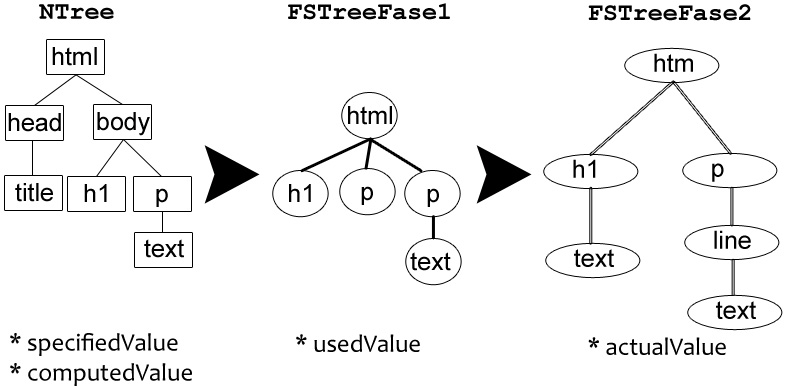
\includegraphics{graphics/transform.jpg}}
\end{figure}

\begin{itemize}
	\item \textit{specifiedValue}: es calculado utilizando el algoritmo cascada de CSS.
	\item \textit{computedValue, usedValue}: es calculado utilizando el comportamiento
	definido en cada propiedad.
\end{itemize}
\end{frame}


\section[Resultados]{Resultados del Proyecto}

\begin{frame}
\begin{center}
	\textbf{\Large Resultados del Proyecto}
\end{center}
\end{frame}


\begin{frame}
\frametitle{Resultados del Proyecto}
Como resultado, se ha desarrollado un Navegador Web con Haskell:

\begin{center}
	\textbf{Simple San Simon Funcional Web Browser}
\end{center}

\textbf{Características:}\\
\begin{itemize}
	\item Trabaja con los protocolos HTTP y File
	\item Soporte para un subconjunto de la gramática de XHTML y CSS
	\item Soporte para 48 propiedades de CSS, que incluye:
	\begin{itemize}
		\item Modificar la dimensión, posición, tipo y estilo de un elemento
		\item Modificar el estilo de un texto
		\item Listas
		\item Generación de contenidos
	\end{itemize}
\end{itemize}
\end{frame}

\section{Conclusiones}

\begin{frame}
\begin{center}
	\textbf{\Large Conclusiones}
\end{center}
\end{frame}

\begin{frame}
\frametitle{Conclusiones}

\begin{block}{}
Se encontró que el lenguaje de programación funcional Haskell fue 
\highlighton{apropiado} y \highlighton{maduro} para el desarrollo de un Navegador Web.
\begin{itemize}
	\item \highlighton{Apropiado}, porque varias partes de la implementación fueron 
	expresadas de mejor manera utilizando mecanismos de la programación funcional.
	\item \highlighton{Maduro}, porque en muchos casos, simplemente se utilizó las librerías
	ya existentes para Haskell.
\end{itemize}
\end{block}

\begin{alertblock}{}
Sin embargo, también se ha tenido varias dificultades en la implementación de algunos
algoritmos, y algunas limitaciones de algunas librerías.
\end{alertblock}
\end{frame}

\subsection{Beneficios del lenguaje}
\begin{frame}
\frametitle{Beneficios del lenguaje}

\begin{block}{}
Al utilizar Haskell como lenguaje de desarrollo, el proyecto se ha beneficiado
con varias de sus características.
\end{block}

\begin{itemize}
	\item Forma rica de definir los tipos de datos. 
%	Permite que el código sea
%	fácil de entender, más expresivo. Ejemplo, tipo de dato \textit{Property}.
	\item Amplia Biblioteca de funciones. 
%	Ejemplo, librería Map y 
%	List (propiedad \textit{white-space}).
	\item Varias formas de definir una función. 
%	Permite que el código sea fácil de
%	entender y expresivo.
	\item Aplicación parcial de funciones.
	\item Definición de módulos. 
%	Permite que el código este organizado en módulos,
%	donde cada modulo tiene funciones publicas para otros módulos.
\end{itemize}
\end{frame}

\subsection{Beneficios de las herramientas y librerías}
\begin{frame}
\frametitle{Beneficios de las Herramientas y Librerías}

\begin{block}{}
Las Herramientas y Librerías utilizadas han jugado un rol importante en la simplificación
de la complejidad en el desarrollo del proyecto.
\end{block}

\textbf{UUAGC}\\
\begin{itemize}
	\item Permite enfocarse en la resolución del problema.
	\item Código compacto (reglas de copiado de UUAGC).
	\item Generar código Haskell sólo de las partes que se necesita.
\end{itemize}
\textbf{uu-parsingLib}\\
\begin{itemize}
	\item Permite que la gramática implementada sea robusta.
	\item Implementar todo en Haskell.
\end{itemize}
\textbf{wxHaskell}\\
\begin{itemize}
	\item Las variables de wxHaskell permitieron implementar el
	diagrama de renderización.
\end{itemize}
\end{frame}

\section[Limitaciones]{Limitaciones del Proyecto}

\begin{frame}
\begin{center}
	\textbf{\Large Limitaciones del Proyecto}
\end{center}
\end{frame}


\begin{frame}
\frametitle{Limitaciones del proyecto}
\begin{block}{}
Este proyecto corresponde simplemente a una pequeña parte de la amplia y compleja área de los
Navegadores Web.
\end{block}

\begin{itemize}
	\item \highlighton{Funcionalidad}\\
	No se dio soporte a:
	\begin{itemize}
		\item Formularios, Tablas y Frames de HTML.
		\item Posicionamiento flotante, absoluto y fijo de CSS.
	\end{itemize}
	\item \highlighton{Limitaciones de la librería wxHaskell}\\
	\begin{itemize}
		\item Color Transparente
		\item Cambio de la fuente de un texto.
	\end{itemize}
\end{itemize}
\end{frame}

\section[Recomendaciones]{Recomendaciones para Trabajos Futuros}

\begin{frame}
\begin{center}
	\textbf{\Large Recomendaciones para Trabajos Futuros}
\end{center}
\end{frame}


\begin{frame}
\frametitle{Recomendaciones para Trabajos Futuros}

\begin{itemize}
	\item Parser de HTML/XHTML + DTD
	\item Extender el soporte para la especificación de CSS.
		\begin{itemize}
			\item Tablas
			\item Posicionamiento flotante, absoluto y fijo
			\item Más propiedades de CSS (sólo se implemento 48 de las 80 propiedades para la pantalla)
		\end{itemize}
	\item Delegar la tarea de dimensionamiento y posicionamiento a la librería gráfica.
	\item Optimizar los algoritmos de renderización del proyecto.
	\item Implementar JavaScript.
\end{itemize}
\end{frame}

\frame{
  \vspace{2cm}
  {\huge Fin de la Presentación}

  \vspace{2cm}
  \begin{flushright}
    Carlos Gomez\\
    \structure{\footnotesize{carliros.g@gmail.com}}\\
	Desarrollo De Navegador Web Con Haskell\\
    \structure{\footnotesize{http://hsbrowser.wordpress.com}}
  \end{flushright}
}

\end{document}
